\documentclass[twoside]{book}

% Packages required by doxygen
\usepackage{fixltx2e}
\usepackage{calc}
\usepackage{doxygen}
\usepackage[export]{adjustbox} % also loads graphicx
\usepackage{graphicx}
\usepackage[utf8]{inputenc}
\usepackage{makeidx}
\usepackage{multicol}
\usepackage{multirow}
\PassOptionsToPackage{warn}{textcomp}
\usepackage{textcomp}
\usepackage[nointegrals]{wasysym}
\usepackage[table]{xcolor}

% Font selection
\usepackage[T1]{fontenc}
\usepackage[scaled=.90]{helvet}
\usepackage{courier}
\usepackage{amssymb}
\usepackage{sectsty}
\renewcommand{\familydefault}{\sfdefault}
\allsectionsfont{%
  \fontseries{bc}\selectfont%
  \color{darkgray}%
}
\renewcommand{\DoxyLabelFont}{%
  \fontseries{bc}\selectfont%
  \color{darkgray}%
}
\newcommand{\+}{\discretionary{\mbox{\scriptsize$\hookleftarrow$}}{}{}}

% Page & text layout
\usepackage{geometry}
\geometry{%
  a4paper,%
  top=2.5cm,%
  bottom=2.5cm,%
  left=2.5cm,%
  right=2.5cm%
}
\tolerance=750
\hfuzz=15pt
\hbadness=750
\setlength{\emergencystretch}{15pt}
\setlength{\parindent}{0cm}
\setlength{\parskip}{3ex plus 2ex minus 2ex}
\makeatletter
\renewcommand{\paragraph}{%
  \@startsection{paragraph}{4}{0ex}{-1.0ex}{1.0ex}{%
    \normalfont\normalsize\bfseries\SS@parafont%
  }%
}
\renewcommand{\subparagraph}{%
  \@startsection{subparagraph}{5}{0ex}{-1.0ex}{1.0ex}{%
    \normalfont\normalsize\bfseries\SS@subparafont%
  }%
}
\makeatother

% Headers & footers
\usepackage{fancyhdr}
\pagestyle{fancyplain}
\fancyhead[LE]{\fancyplain{}{\bfseries\thepage}}
\fancyhead[CE]{\fancyplain{}{}}
\fancyhead[RE]{\fancyplain{}{\bfseries\leftmark}}
\fancyhead[LO]{\fancyplain{}{\bfseries\rightmark}}
\fancyhead[CO]{\fancyplain{}{}}
\fancyhead[RO]{\fancyplain{}{\bfseries\thepage}}
\fancyfoot[LE]{\fancyplain{}{}}
\fancyfoot[CE]{\fancyplain{}{}}
\fancyfoot[RE]{\fancyplain{}{\bfseries\scriptsize Generated by Doxygen }}
\fancyfoot[LO]{\fancyplain{}{\bfseries\scriptsize Generated by Doxygen }}
\fancyfoot[CO]{\fancyplain{}{}}
\fancyfoot[RO]{\fancyplain{}{}}
\renewcommand{\footrulewidth}{0.4pt}
\renewcommand{\chaptermark}[1]{%
  \markboth{#1}{}%
}
\renewcommand{\sectionmark}[1]{%
  \markright{\thesection\ #1}%
}

% Indices & bibliography
\usepackage{natbib}
\usepackage[titles]{tocloft}
\setcounter{tocdepth}{3}
\setcounter{secnumdepth}{5}
\makeindex

% Hyperlinks (required, but should be loaded last)
\usepackage{ifpdf}
\ifpdf
  \usepackage[pdftex,pagebackref=true]{hyperref}
\else
  \usepackage[ps2pdf,pagebackref=true]{hyperref}
\fi
\hypersetup{%
  colorlinks=true,%
  linkcolor=blue,%
  citecolor=blue,%
  unicode%
}

% Custom commands
\newcommand{\clearemptydoublepage}{%
  \newpage{\pagestyle{empty}\cleardoublepage}%
}

\usepackage{caption}
\captionsetup{labelsep=space,justification=centering,font={bf},singlelinecheck=off,skip=4pt,position=top}

%===== C O N T E N T S =====

\begin{document}

% Titlepage & ToC
\hypersetup{pageanchor=false,
             bookmarksnumbered=true,
             pdfencoding=unicode
            }
\pagenumbering{roman}
\begin{titlepage}
\vspace*{7cm}
\begin{center}%
{\Large Lane Detection and Prediction }\\
\vspace*{1cm}
{\large Generated by Doxygen 1.8.11}\\
\end{center}
\end{titlepage}
\clearemptydoublepage
\tableofcontents
\clearemptydoublepage
\pagenumbering{arabic}
\hypersetup{pageanchor=true}

%--- Begin generated contents ---
\chapter{Hierarchical Index}
\section{Class Hierarchy}
This inheritance list is sorted roughly, but not completely, alphabetically\+:\begin{DoxyCompactList}
\item \contentsline{section}{Lane\+Detector}{\pageref{classLaneDetector}}{}
\begin{DoxyCompactList}
\item \contentsline{section}{Lane\+Predictor}{\pageref{classLanePredictor}}{}
\end{DoxyCompactList}
\end{DoxyCompactList}

\chapter{Class Index}
\section{Class List}
Here are the classes, structs, unions and interfaces with brief descriptions\+:\begin{DoxyCompactList}
\item\contentsline{section}{\hyperlink{classLaneDetector}{Lane\+Detector} \\*Class for lane detector.\+Carries all the functions related to detect the yellow and white lanes }{\pageref{classLaneDetector}}{}
\item\contentsline{section}{\hyperlink{classLanePredictor}{Lane\+Predictor} \\*Class for lane predictor }{\pageref{classLanePredictor}}{}
\end{DoxyCompactList}

\chapter{File Index}
\section{File List}
Here is a list of all documented files with brief descriptions\+:\begin{DoxyCompactList}
\item\contentsline{section}{/home/bob/\+Bob\+\_\+old/\+Mathworks/\+Mid\+Term\+\_\+\+Lane\+Detection/include/{\bfseries Lane\+Detector.\+hpp} }{\pageref{LaneDetector_8hpp}}{}
\item\contentsline{section}{/home/bob/\+Bob\+\_\+old/\+Mathworks/\+Mid\+Term\+\_\+\+Lane\+Detection/include/{\bfseries Lane\+Predictor.\+hpp} }{\pageref{LanePredictor_8hpp}}{}
\item\contentsline{section}{/home/bob/\+Bob\+\_\+old/\+Mathworks/\+Mid\+Term\+\_\+\+Lane\+Detection/test/\hyperlink{test_8cpp}{test.\+cpp} \\*Mid-\/\+Term Project (with partner component) }{\pageref{test_8cpp}}{}
\end{DoxyCompactList}

\chapter{Class Documentation}
\hypertarget{classLaneDetector}{}\section{Lane\+Detector Class Reference}
\label{classLaneDetector}\index{Lane\+Detector@{Lane\+Detector}}


Class for lane detector.\+Carries all the functions related to detect the yellow and white lanes.  




{\ttfamily \#include $<$Lane\+Detector.\+hpp$>$}



Inheritance diagram for Lane\+Detector\+:
% FIG 0
\subsection*{Public Member Functions}
\begin{DoxyCompactItemize}
\item 
cv\+::\+Mat \hyperlink{classLaneDetector_aa29c19c559518b81897c90e545c3aae1}{read\+Frame} (int frame\+\_\+number)
\begin{DoxyCompactList}\small\item\em Reads a frame. \end{DoxyCompactList}\item 
cv\+::\+Mat \hyperlink{classLaneDetector_a5ad301b4756ae451f49b43947771c02f}{roi\+Mask\+Selection} (cv\+::\+Mat input\+\_\+image)
\begin{DoxyCompactList}\small\item\em \{ selects a trapezoidal region in given image\} \end{DoxyCompactList}\item 
cv\+::\+Mat \hyperlink{classLaneDetector_a2caab27786b6168a125313aa2c36434b}{edge\+Detector} (cv\+::\+Mat thresh\+\_\+image)
\begin{DoxyCompactList}\small\item\em \{ applies canny edge detections on given image \} \end{DoxyCompactList}\item 
std\+::vector$<$ std\+::vector$<$ cv\+::\+Vec4i $>$ $>$ \hyperlink{classLaneDetector_a88ab13cba16e8e817b6d913d5acd681b}{hough\+Transform} (cv\+::\+Mat)
\begin{DoxyCompactList}\small\item\em \{ Applies Hough Transform and classifies lanes based on slopes \} \end{DoxyCompactList}\item 
cv\+::\+Vec4d \hyperlink{classLaneDetector_a8cb3e5505c760fa460a01f8eacbb3f1c}{line\+Fitting} (std\+::vector$<$ cv\+::\+Vec4i $>$, cv\+::\+Mat)
\begin{DoxyCompactList}\small\item\em \{ curve fits a line using multiple lines \} \end{DoxyCompactList}\end{DoxyCompactItemize}


\subsection{Detailed Description}
Class for lane detector.\+Carries all the functions related to detect the yellow and white lanes. 

\subsection{Member Function Documentation}
\index{Lane\+Detector@{Lane\+Detector}!edge\+Detector@{edge\+Detector}}
\index{edge\+Detector@{edge\+Detector}!Lane\+Detector@{Lane\+Detector}}
\subsubsection[{\texorpdfstring{edge\+Detector(cv\+::\+Mat thresh\+\_\+image)}{edgeDetector(cv::Mat thresh_image)}}]{\setlength{\rightskip}{0pt plus 5cm}cv\+::\+Mat Lane\+Detector\+::edge\+Detector (
\begin{DoxyParamCaption}
\item[{cv\+::\+Mat}]{roi\+\_\+image}
\end{DoxyParamCaption}
)}\hypertarget{classLaneDetector_a2caab27786b6168a125313aa2c36434b}{}\label{classLaneDetector_a2caab27786b6168a125313aa2c36434b}


\{ applies canny edge detections on given image \} 

reads image and applys canny edge detecting. This file is a library file to implement Canny edge detection algorithm on the input frame. The kernel size for the edge detection algorithm is chosen as 3.


\begin{DoxyParams}[1]{Parameters}
\mbox{\tt in}  & {\em thresh\+\_\+image} & The thresh image\\
\hline
\end{DoxyParams}
\begin{DoxyReturn}{Returns}
\{ image containing all the edges \}
\end{DoxyReturn}

\begin{DoxyParams}[1]{Parameters}
\mbox{\tt in}  & {\em roi\+\_\+image} & cv\+::\+Mat \\
\hline
\end{DoxyParams}
\begin{DoxyReturn}{Returns}
edge\+\_\+image cv\+::\+Mat 
\end{DoxyReturn}
\index{Lane\+Detector@{Lane\+Detector}!hough\+Transform@{hough\+Transform}}
\index{hough\+Transform@{hough\+Transform}!Lane\+Detector@{Lane\+Detector}}
\subsubsection[{\texorpdfstring{hough\+Transform(cv\+::\+Mat)}{houghTransform(cv::Mat)}}]{\setlength{\rightskip}{0pt plus 5cm}std\+::vector$<$ std\+::vector$<$ cv\+::\+Vec4i $>$ $>$ Lane\+Detector\+::hough\+Transform (
\begin{DoxyParamCaption}
\item[{cv\+::\+Mat}]{roi\+\_\+image}
\end{DoxyParamCaption}
)}\hypertarget{classLaneDetector_a88ab13cba16e8e817b6d913d5acd681b}{}\label{classLaneDetector_a88ab13cba16e8e817b6d913d5acd681b}


\{ Applies Hough Transform and classifies lanes based on slopes \} 

reads image and return lane points This file is a library file to implement hough tranform to find lines in the edged image then classify detected lines into left and right lane


\begin{DoxyParams}[1]{Parameters}
\mbox{\tt in}  & {\em \{} & cv\+::\+Mat edged Image \}\\
\hline
\end{DoxyParams}
\begin{DoxyReturn}{Returns}
\{ vector containing all points of left and right lanes \}
\end{DoxyReturn}

\begin{DoxyParams}[1]{Parameters}
\mbox{\tt in}  & {\em roi\+\_\+image} & cv\+::\+Mat \\
\hline
\end{DoxyParams}
\begin{DoxyReturn}{Returns}
lanes std\+::vector$<$std\+::vector$<$cv\+::\+Vec4i$>$ $>$ 
\end{DoxyReturn}
\index{Lane\+Detector@{Lane\+Detector}!line\+Fitting@{line\+Fitting}}
\index{line\+Fitting@{line\+Fitting}!Lane\+Detector@{Lane\+Detector}}
\subsubsection[{\texorpdfstring{line\+Fitting(std\+::vector$<$ cv\+::\+Vec4i $>$, cv\+::\+Mat)}{lineFitting(std::vector< cv::Vec4i >, cv::Mat)}}]{\setlength{\rightskip}{0pt plus 5cm}cv\+::\+Vec4d Lane\+Detector\+::line\+Fitting (
\begin{DoxyParamCaption}
\item[{std\+::vector$<$ cv\+::\+Vec4i $>$}]{line\+Vector, }
\item[{cv\+::\+Mat}]{input\+Image}
\end{DoxyParamCaption}
)}\hypertarget{classLaneDetector_a8cb3e5505c760fa460a01f8eacbb3f1c}{}\label{classLaneDetector_a8cb3e5505c760fa460a01f8eacbb3f1c}


\{ curve fits a line using multiple lines \} 

fits a line over given input points This file is a library file to fit lines over the detected lines on the input image.


\begin{DoxyParams}[1]{Parameters}
\mbox{\tt in}  & {\em lines} & \{vector containing lines \} \\
\hline
\mbox{\tt in}  & {\em cv\+::\+Mat} & \{ input\+\_\+image \}\\
\hline
\end{DoxyParams}
\begin{DoxyReturn}{Returns}
\{ two ends of the fit line \}
\end{DoxyReturn}

\begin{DoxyParams}[1]{Parameters}
\mbox{\tt in}  & {\em line\+Vector} & The line vector \\
\hline
\mbox{\tt in}  & {\em input\+Image} & The input image\\
\hline
\end{DoxyParams}
\begin{DoxyReturn}{Returns}
\{ return two points based one fit line\} 
\end{DoxyReturn}
\index{Lane\+Detector@{Lane\+Detector}!read\+Frame@{read\+Frame}}
\index{read\+Frame@{read\+Frame}!Lane\+Detector@{Lane\+Detector}}
\subsubsection[{\texorpdfstring{read\+Frame(int frame\+\_\+number)}{readFrame(int frame_number)}}]{\setlength{\rightskip}{0pt plus 5cm}cv\+::\+Mat Lane\+Detector\+::read\+Frame (
\begin{DoxyParamCaption}
\item[{int}]{frame\+\_\+number}
\end{DoxyParamCaption}
)}\hypertarget{classLaneDetector_aa29c19c559518b81897c90e545c3aae1}{}\label{classLaneDetector_aa29c19c559518b81897c90e545c3aae1}


Reads a frame. 

\mbox{[}\hyperlink{classLaneDetector_aa29c19c559518b81897c90e545c3aae1}{Lane\+Detector\+::read\+Frame}\mbox{]} This file is a library file to read image frames from the input image as per the frame number given as argument.


\begin{DoxyParams}[1]{Parameters}
\mbox{\tt in}  & {\em frame\+\_\+number} & The frame number\\
\hline
\end{DoxyParams}
\begin{DoxyReturn}{Returns}
\{ frame of the given frame index\}
\end{DoxyReturn}

\begin{DoxyParams}[1]{Parameters}
\mbox{\tt in}  & {\em frame\+\_\+number} & \mbox{[}int\mbox{]} \\
\hline
\end{DoxyParams}
\begin{DoxyReturn}{Returns}
frame \mbox{[}cv\+::\+Mat\mbox{]} 
\end{DoxyReturn}
\index{Lane\+Detector@{Lane\+Detector}!roi\+Mask\+Selection@{roi\+Mask\+Selection}}
\index{roi\+Mask\+Selection@{roi\+Mask\+Selection}!Lane\+Detector@{Lane\+Detector}}
\subsubsection[{\texorpdfstring{roi\+Mask\+Selection(cv\+::\+Mat input\+\_\+image)}{roiMaskSelection(cv::Mat input_image)}}]{\setlength{\rightskip}{0pt plus 5cm}cv\+::\+Mat Lane\+Detector\+::roi\+Mask\+Selection (
\begin{DoxyParamCaption}
\item[{cv\+::\+Mat}]{hsv\+\_\+threshold}
\end{DoxyParamCaption}
)}\hypertarget{classLaneDetector_a5ad301b4756ae451f49b43947771c02f}{}\label{classLaneDetector_a5ad301b4756ae451f49b43947771c02f}


\{ selects a trapezoidal region in given image\} 

\hyperlink{classLaneDetector_a5ad301b4756ae451f49b43947771c02f}{Lane\+Detector\+::roi\+Mask\+Selection} This file is a library file to mask the input image with region of interest.


\begin{DoxyParams}[1]{Parameters}
\mbox{\tt in}  & {\em input\+\_\+image} & The input image\\
\hline
\end{DoxyParams}
\begin{DoxyReturn}{Returns}
\{ retuns region of interest in given image \}
\end{DoxyReturn}

\begin{DoxyParams}[1]{Parameters}
\mbox{\tt in}  & {\em hsv\+\_\+threshold} & cv\+::\+Mat \\
\hline
\end{DoxyParams}
\begin{DoxyReturn}{Returns}
roi cv\+::\+Mat 
\end{DoxyReturn}


The documentation for this class was generated from the following files\+:\begin{DoxyCompactItemize}
\item 
/home/mp/808\+X\+Work\+Space/\+Midterm/\+Mid\+Term\+\_\+\+Lane\+Detection/include/Lane\+Detector.\+hpp\item 
/home/mp/808\+X\+Work\+Space/\+Midterm/\+Mid\+Term\+\_\+\+Lane\+Detection/app/\hyperlink{edgeDetector_8cpp}{edge\+Detector.\+cpp}\item 
/home/mp/808\+X\+Work\+Space/\+Midterm/\+Mid\+Term\+\_\+\+Lane\+Detection/app/\hyperlink{houghTransform_8cpp}{hough\+Transform.\+cpp}\item 
/home/mp/808\+X\+Work\+Space/\+Midterm/\+Mid\+Term\+\_\+\+Lane\+Detection/app/\hyperlink{lineFitting_8cpp}{line\+Fitting.\+cpp}\item 
/home/mp/808\+X\+Work\+Space/\+Midterm/\+Mid\+Term\+\_\+\+Lane\+Detection/app/\hyperlink{readFrame_8cpp}{read\+Frame.\+cpp}\item 
/home/mp/808\+X\+Work\+Space/\+Midterm/\+Mid\+Term\+\_\+\+Lane\+Detection/app/\hyperlink{roiMaskSelection_8cpp}{roi\+Mask\+Selection.\+cpp}\end{DoxyCompactItemize}

\hypertarget{classLanePredictor}{}\section{Lane\+Predictor Class Reference}
\label{classLanePredictor}\index{Lane\+Predictor@{Lane\+Predictor}}


Class for lane predictor.  




{\ttfamily \#include $<$Lane\+Predictor.\+hpp$>$}



Inheritance diagram for Lane\+Predictor\+:
\nopagebreak
\begin{figure}[H]
\begin{center}
\leavevmode
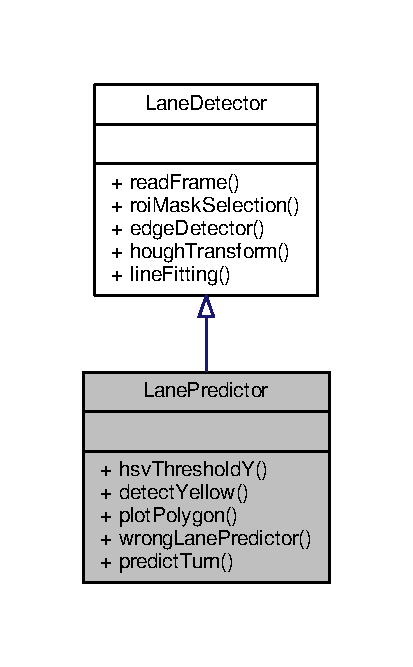
\includegraphics[width=198pt]{classLanePredictor__inherit__graph}
\end{center}
\end{figure}


Collaboration diagram for Lane\+Predictor\+:
\nopagebreak
\begin{figure}[H]
\begin{center}
\leavevmode
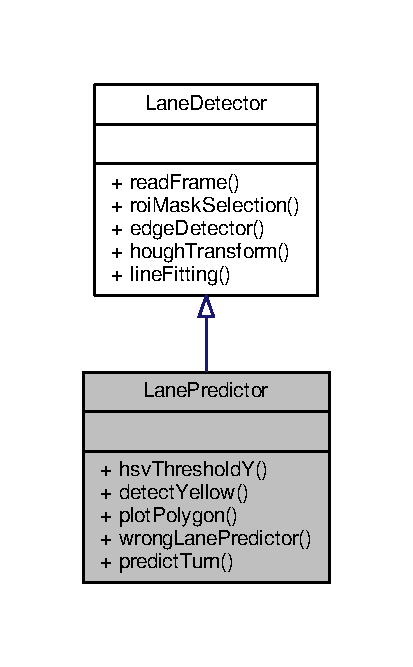
\includegraphics[width=198pt]{classLanePredictor__coll__graph}
\end{center}
\end{figure}
\subsection*{Public Member Functions}
\begin{DoxyCompactItemize}
\item 
cv\+::\+Mat \hyperlink{classLanePredictor_ada11760da395c1d2f9e6117212659742}{hsv\+ThresholdY} (cv\+::\+Mat frameP)
\begin{DoxyCompactList}\small\item\em \{ to threshold the image to get only yellow lanes\} \end{DoxyCompactList}\item 
cv\+::\+Vec4d \hyperlink{classLanePredictor_a2ab03a2ebd0cca2c27a5773533f16dd3}{detect\+Yellow} (cv\+::\+Mat)
\begin{DoxyCompactList}\small\item\em \{ It finds the yellow lane \} \end{DoxyCompactList}\item 
cv\+::\+Mat \hyperlink{classLanePredictor_ab793993ceb4f18d3fcd2b57779fef859}{plot\+Polygon} (cv\+::\+Mat, cv\+::\+Vec4d, cv\+::\+Vec4d)
\begin{DoxyCompactList}\small\item\em \{ to plot a polygon over detected lanes \} \end{DoxyCompactList}\item 
std\+::string \hyperlink{classLanePredictor_ac930fa52cdede9afa25bbf7cafd8c6b5}{wrong\+Lane\+Predictor} (cv\+::\+Vec4d)
\begin{DoxyCompactList}\small\item\em \{predict if vehicle is on wrong lane \} \end{DoxyCompactList}\item 
std\+::string \hyperlink{classLanePredictor_a9b72c2dfa77992f7f8e229c3a67103f7}{predict\+Turn} (cv\+::\+Vec4d, cv\+::\+Vec4d, cv\+::\+Mat)
\begin{DoxyCompactList}\small\item\em \{function which calculates vanishing points and predicts turn \} \end{DoxyCompactList}\end{DoxyCompactItemize}


\subsection{Detailed Description}
Class for lane predictor. 

\subsection{Member Function Documentation}
\index{Lane\+Predictor@{Lane\+Predictor}!detect\+Yellow@{detect\+Yellow}}
\index{detect\+Yellow@{detect\+Yellow}!Lane\+Predictor@{Lane\+Predictor}}
\subsubsection[{\texorpdfstring{detect\+Yellow(cv\+::\+Mat)}{detectYellow(cv::Mat)}}]{\setlength{\rightskip}{0pt plus 5cm}cv\+::\+Vec4d Lane\+Predictor\+::detect\+Yellow (
\begin{DoxyParamCaption}
\item[{cv\+::\+Mat}]{frame}
\end{DoxyParamCaption}
)}\hypertarget{classLanePredictor_a2ab03a2ebd0cca2c27a5773533f16dd3}{}\label{classLanePredictor_a2ab03a2ebd0cca2c27a5773533f16dd3}


\{ It finds the yellow lane \} 

\hyperlink{classLanePredictor_a2ab03a2ebd0cca2c27a5773533f16dd3}{Lane\+Predictor\+::detect\+Yellow}, returns end points of yellow lanes after curve fitting on points found from hough transform. This file is a library file to detect yellow lanes as per hsvthreshold output. This file inherits hsv\+ThresholdY, edge\+Detector, roi\+Mask\+Selection and line\+Fitting functions from \hyperlink{classLaneDetector}{Lane\+Detector} Class.


\begin{DoxyParams}[1]{Parameters}
\mbox{\tt in}  & {\em \{} & thresholded image \}\\
\hline
\end{DoxyParams}
\begin{DoxyReturn}{Returns}
\{ end points of the yellow lines \}
\end{DoxyReturn}

\begin{DoxyParams}[1]{Parameters}
\mbox{\tt in}  & {\em frame} & \mbox{[}cv\+::\+Mat\mbox{]} \\
\hline
\end{DoxyParams}
\begin{DoxyReturn}{Returns}
\mbox{[}cv\+::\+Vect4d\mbox{]} 
\end{DoxyReturn}
\index{Lane\+Predictor@{Lane\+Predictor}!hsv\+ThresholdY@{hsv\+ThresholdY}}
\index{hsv\+ThresholdY@{hsv\+ThresholdY}!Lane\+Predictor@{Lane\+Predictor}}
\subsubsection[{\texorpdfstring{hsv\+Threshold\+Y(cv\+::\+Mat frame\+P)}{hsvThresholdY(cv::Mat frameP)}}]{\setlength{\rightskip}{0pt plus 5cm}cv\+::\+Mat Lane\+Predictor\+::hsv\+ThresholdY (
\begin{DoxyParamCaption}
\item[{cv\+::\+Mat}]{frame}
\end{DoxyParamCaption}
)}\hypertarget{classLanePredictor_ada11760da395c1d2f9e6117212659742}{}\label{classLanePredictor_ada11760da395c1d2f9e6117212659742}


\{ to threshold the image to get only yellow lanes\} 

\hyperlink{classLanePredictor_ada11760da395c1d2f9e6117212659742}{Lane\+Predictor\+::hsv\+ThresholdY} Split B\+GR image into H\+SV planes and apply threshold on each plane to detect Yellow Lanes.


\begin{DoxyParams}[1]{Parameters}
\mbox{\tt in}  & {\em frameP} & The frame of the video\\
\hline
\end{DoxyParams}
\begin{DoxyReturn}{Returns}
\{ thresholded image \}
\end{DoxyReturn}

\begin{DoxyParams}[1]{Parameters}
\mbox{\tt in}  & {\em frame} & \mbox{[}cv\+::\+Mat\mbox{]} \\
\hline
\end{DoxyParams}
\begin{DoxyReturn}{Returns}
threshold\+\_\+image \mbox{[}cv\+::\+Mat\mbox{]} 
\end{DoxyReturn}
\index{Lane\+Predictor@{Lane\+Predictor}!plot\+Polygon@{plot\+Polygon}}
\index{plot\+Polygon@{plot\+Polygon}!Lane\+Predictor@{Lane\+Predictor}}
\subsubsection[{\texorpdfstring{plot\+Polygon(cv\+::\+Mat, cv\+::\+Vec4d, cv\+::\+Vec4d)}{plotPolygon(cv::Mat, cv::Vec4d, cv::Vec4d)}}]{\setlength{\rightskip}{0pt plus 5cm}cv\+::\+Mat Lane\+Predictor\+::plot\+Polygon (
\begin{DoxyParamCaption}
\item[{cv\+::\+Mat}]{input\+\_\+image, }
\item[{cv\+::\+Vec4d}]{yellow\+\_\+lanes, }
\item[{cv\+::\+Vec4d}]{white\+\_\+lanes}
\end{DoxyParamCaption}
)}\hypertarget{classLanePredictor_ab793993ceb4f18d3fcd2b57779fef859}{}\label{classLanePredictor_ab793993ceb4f18d3fcd2b57779fef859}


\{ to plot a polygon over detected lanes \} 

\hyperlink{classLanePredictor_ab793993ceb4f18d3fcd2b57779fef859}{Lane\+Predictor\+::plot\+Polygon} This file is a library file to plot a polygon over detected lanes on the output frame.


\begin{DoxyParams}[1]{Parameters}
\mbox{\tt in}  & {\em \{} & image to plot lanes\} \\
\hline
\mbox{\tt in}  & {\em \{} & left lanes \} \\
\hline
\mbox{\tt in}  & {\em \{} & right lanes \}\\
\hline
\end{DoxyParams}
\begin{DoxyReturn}{Returns}
\{Image with polygon plot \}
\end{DoxyReturn}

\begin{DoxyParams}[1]{Parameters}
\mbox{\tt in}  & {\em input\+\_\+image} & \mbox{[}cv\+::\+Mat\mbox{]} \\
\hline
\mbox{\tt in}  & {\em yellow\+\_\+lanes} & \mbox{[}cv\+::\+Vec4d\mbox{]} \\
\hline
\mbox{\tt in}  & {\em white\+\_\+lanes} & \mbox{[}cv\+::\+Vec4d\mbox{]} \\
\hline
\end{DoxyParams}
\begin{DoxyReturn}{Returns}
output \mbox{[}cv\+::\+Mat\mbox{]} 
\end{DoxyReturn}
\index{Lane\+Predictor@{Lane\+Predictor}!predict\+Turn@{predict\+Turn}}
\index{predict\+Turn@{predict\+Turn}!Lane\+Predictor@{Lane\+Predictor}}
\subsubsection[{\texorpdfstring{predict\+Turn(cv\+::\+Vec4d, cv\+::\+Vec4d, cv\+::\+Mat)}{predictTurn(cv::Vec4d, cv::Vec4d, cv::Mat)}}]{\setlength{\rightskip}{0pt plus 5cm}std\+::string Lane\+Predictor\+::predict\+Turn (
\begin{DoxyParamCaption}
\item[{cv\+::\+Vec4d}]{left\+\_\+lines, }
\item[{cv\+::\+Vec4d}]{right\+\_\+lines, }
\item[{cv\+::\+Mat}]{input\+\_\+image}
\end{DoxyParamCaption}
)}\hypertarget{classLanePredictor_a9b72c2dfa77992f7f8e229c3a67103f7}{}\label{classLanePredictor_a9b72c2dfa77992f7f8e229c3a67103f7}


\{function which calculates vanishing points and predicts turn \} 

\mbox{[}\hyperlink{classLanePredictor_a9b72c2dfa77992f7f8e229c3a67103f7}{Lane\+Predictor\+::predict\+Turn}\mbox{]} This file is a library file to predict turns based on the concept of vanishing point.


\begin{DoxyParams}[1]{Parameters}
\mbox{\tt in}  & {\em \{} & left lanes end points\} \\
\hline
\mbox{\tt in}  & {\em \{} & right lane end points \} \\
\hline
\mbox{\tt in}  & {\em \{} & Output Image \}\\
\hline
\end{DoxyParams}
\begin{DoxyReturn}{Returns}
\{Output Image with predicted turns text \}
\end{DoxyReturn}

\begin{DoxyParams}[1]{Parameters}
\mbox{\tt in}  & {\em left\+\_\+lines} & \mbox{[}cv\+::\+Vec4d\mbox{]} \\
\hline
\mbox{\tt in}  & {\em right\+\_\+lines} & \mbox{[}cv\+::\+Vec4d\mbox{]} \\
\hline
\mbox{\tt in}  & {\em input\+\_\+image} & \mbox{[}cv\+::\+Mat\mbox{]} \\
\hline
\end{DoxyParams}
\begin{DoxyReturn}{Returns}
\mbox{[}in\mbox{]} input\+\_\+image \mbox{[}cv\+::\+Mat\mbox{]} 
\end{DoxyReturn}
\index{Lane\+Predictor@{Lane\+Predictor}!wrong\+Lane\+Predictor@{wrong\+Lane\+Predictor}}
\index{wrong\+Lane\+Predictor@{wrong\+Lane\+Predictor}!Lane\+Predictor@{Lane\+Predictor}}
\subsubsection[{\texorpdfstring{wrong\+Lane\+Predictor(cv\+::\+Vec4d)}{wrongLanePredictor(cv::Vec4d)}}]{\setlength{\rightskip}{0pt plus 5cm}std\+::string Lane\+Predictor\+::wrong\+Lane\+Predictor (
\begin{DoxyParamCaption}
\item[{cv\+::\+Vec4d}]{yellow\+\_\+line}
\end{DoxyParamCaption}
)}\hypertarget{classLanePredictor_ac930fa52cdede9afa25bbf7cafd8c6b5}{}\label{classLanePredictor_ac930fa52cdede9afa25bbf7cafd8c6b5}


\{predict if vehicle is on wrong lane \} 

\mbox{[}\hyperlink{classLanePredictor_ac930fa52cdede9afa25bbf7cafd8c6b5}{Lane\+Predictor\+::wrong\+Lane\+Predictor} description\mbox{]} This file is a library file to predict vehicle position based on yellow lane w.\+r.\+t. the frame size. (Assuming Right-\/\+Hand Drive System)


\begin{DoxyParams}[1]{Parameters}
\mbox{\tt in}  & {\em \{} & yellow lane end points\}\\
\hline
\end{DoxyParams}
\begin{DoxyReturn}{Returns}
\{string indicating the lane\}
\end{DoxyReturn}

\begin{DoxyParams}[1]{Parameters}
\mbox{\tt in}  & {\em yellow\+\_\+line} & \mbox{[}cv\+::\+Vec4d\mbox{]} \\
\hline
\end{DoxyParams}
\begin{DoxyReturn}{Returns}
lane\+\_\+indicator \mbox{[}string\mbox{]} 
\end{DoxyReturn}


The documentation for this class was generated from the following files\+:\begin{DoxyCompactItemize}
\item 
/home/bob/\+Bob\+\_\+old/\+Mathworks/\+Mid\+Term\+\_\+\+Lane\+Detection/include/Lane\+Predictor.\+hpp\item 
/home/bob/\+Bob\+\_\+old/\+Mathworks/\+Mid\+Term\+\_\+\+Lane\+Detection/app/Lane\+Predictor.\+cpp\end{DoxyCompactItemize}

\chapter{File Documentation}
\hypertarget{test_8cpp}{}\section{/home/mp/808\+X\+Work\+Space/\+Midterm/\+Mid\+Term\+\_\+\+Lane\+Detection/test/test.cpp File Reference}
\label{test_8cpp}\index{/home/mp/808\+X\+Work\+Space/\+Midterm/\+Mid\+Term\+\_\+\+Lane\+Detection/test/test.\+cpp@{/home/mp/808\+X\+Work\+Space/\+Midterm/\+Mid\+Term\+\_\+\+Lane\+Detection/test/test.\+cpp}}


Mid-\/\+Term Project (with partner component)  


{\ttfamily \#include $<$gtest/gtest.\+h$>$}\\*
{\ttfamily \#include \char`\"{}../include/\+Lane\+Detector.\+hpp\char`\"{}}\\*
Include dependency graph for test.\+cpp\+:
% FIG 0
\subsection*{Functions}
\begin{DoxyCompactItemize}
\item 
std\+::string \hyperlink{test_8cpp_af7356526639daa99fbc6efb968b2fea7}{Lane\+Testingfor\+Turn} (int framenumber)\hypertarget{test_8cpp_af7356526639daa99fbc6efb968b2fea7}{}\label{test_8cpp_af7356526639daa99fbc6efb968b2fea7}

\begin{DoxyCompactList}\small\item\em To test if the lanes are detected in the given Frame. \end{DoxyCompactList}\item 
int \hyperlink{test_8cpp_a755b5c12fc96a5c43c9f3e5770218951}{Lane\+Testing} (int framenumber)\hypertarget{test_8cpp_a755b5c12fc96a5c43c9f3e5770218951}{}\label{test_8cpp_a755b5c12fc96a5c43c9f3e5770218951}

\begin{DoxyCompactList}\small\item\em To test if the lanes are detected in the given Frame. \end{DoxyCompactList}\item 
\hyperlink{test_8cpp_ad71fa10af78b3c1d7a6ff06e6d1ce111}{T\+E\+ST} (Lane\+Test, lane\+\_\+detected)\hypertarget{test_8cpp_ad71fa10af78b3c1d7a6ff06e6d1ce111}{}\label{test_8cpp_ad71fa10af78b3c1d7a6ff06e6d1ce111}

\begin{DoxyCompactList}\small\item\em Test case to test if lane is detected. \end{DoxyCompactList}\item 
\hyperlink{test_8cpp_ab2c1aa02329a8611f8fd9005c598c7a3}{T\+E\+ST} (Lane\+Test, Lane\+\_\+correct)\hypertarget{test_8cpp_ab2c1aa02329a8611f8fd9005c598c7a3}{}\label{test_8cpp_ab2c1aa02329a8611f8fd9005c598c7a3}

\begin{DoxyCompactList}\small\item\em Test case to test if wrong lane detection is working. \end{DoxyCompactList}\item 
\hyperlink{test_8cpp_a5160c10a881093d0e77ed9fd34b66ea3}{T\+E\+ST} (Lane\+Test, lane\+\_\+wrong)\hypertarget{test_8cpp_a5160c10a881093d0e77ed9fd34b66ea3}{}\label{test_8cpp_a5160c10a881093d0e77ed9fd34b66ea3}

\begin{DoxyCompactList}\small\item\em Test case to test if wrong lane detection is working. \end{DoxyCompactList}\item 
\hyperlink{test_8cpp_ad6f42a29b11367b38cd4c5495ff2d751}{T\+E\+ST} (Lane\+Test, no\+\_\+turn)\hypertarget{test_8cpp_ad6f42a29b11367b38cd4c5495ff2d751}{}\label{test_8cpp_ad6f42a29b11367b38cd4c5495ff2d751}

\begin{DoxyCompactList}\small\item\em Test cases to test if lane is detected and if the lane is going straight. \end{DoxyCompactList}\item 
\hyperlink{test_8cpp_a8561acb13779f6ced5a6775d94f08438}{T\+E\+ST} (Lane\+Test, right\+\_\+turn)\hypertarget{test_8cpp_a8561acb13779f6ced5a6775d94f08438}{}\label{test_8cpp_a8561acb13779f6ced5a6775d94f08438}

\begin{DoxyCompactList}\small\item\em Test cases to test if lane is detected and if the lane is turning right. \end{DoxyCompactList}\item 
\hyperlink{test_8cpp_a39dc9bdc0f27bb5d67f13edccc8cad0f}{T\+E\+ST} (Lane\+Test, left\+\_\+turn)\hypertarget{test_8cpp_a39dc9bdc0f27bb5d67f13edccc8cad0f}{}\label{test_8cpp_a39dc9bdc0f27bb5d67f13edccc8cad0f}

\begin{DoxyCompactList}\small\item\em Test cases to test if lane is detected and if the lane is turning left. \end{DoxyCompactList}\end{DoxyCompactItemize}


\subsection{Detailed Description}
Mid-\/\+Term Project (with partner component) 

\begin{DoxyAuthor}{Authors}
Mayank Pathak and Bhargav Dandamudi 
\end{DoxyAuthor}
\begin{DoxyVersion}{Version}
1.\+0 
\end{DoxyVersion}
\begin{DoxyCopyright}{Copyright}
(c) M\+IT License 2018 Mayank Pathak, Bhargav Dandamudi
\end{DoxyCopyright}
\hypertarget{test_8cpp_DESCRIPTION}{}\subsection{D\+E\+S\+C\+R\+I\+P\+T\+I\+ON}\label{test_8cpp_DESCRIPTION}
This is the header file to declare all the class variables and functions that will be used for the Lane Detection Implementation.

\+: This program needs the following libraries in order to execute properly\+: Open\+CV, String, I\+Ostream, vector 
%--- End generated contents ---

% Index
\backmatter
\newpage
\phantomsection
\clearemptydoublepage
\addcontentsline{toc}{chapter}{Index}
\printindex

\end{document}
